\documentclass[UTF8]{article}
\usepackage{graphicx}
\usepackage{subfigure}
\usepackage{amsmath}
\usepackage{makecell}
\usepackage[utf8]{inputenc}
\usepackage[space]{ctex} %中文包
\usepackage{listings} %放代码
\usepackage{xcolor} %代码着色宏包
\usepackage{CJK} %显示中文宏包
\usepackage{float}

\definecolor{mygreen}{rgb}{0,0.6,0}
\definecolor{mygray}{rgb}{0.5,0.5,0.5}
\definecolor{mymauve}{rgb}{0.58,0,0.82}
\lstset{
	backgroundcolor=\color{white}, 
	basicstyle = \footnotesize,       
	breakatwhitespace = false,        
	breaklines = true,                 
	captionpos = b,                    
	commentstyle = \color{mygreen}\bfseries,
	extendedchars = false,
	frame = shadowbox, 
	framerule=0.5pt,
	keepspaces=true,
	keywordstyle=\color{blue}\bfseries, % keyword style
	language = C++,                     % the language of code
	otherkeywords={string}, 
	numbers=left, 
	numbersep=5pt,
	numberstyle=\tiny\color{mygray},
	rulecolor=\color{black},         
	showspaces=false,  
	showstringspaces=false, 
	showtabs=false,    
	stepnumber=1,         
	stringstyle=\color{mymauve},        % string literal style
	tabsize=4,          
	title=\lstname           
}


%画图包
\usepackage{tikz}
%画图背景包
\usetikzlibrary{backgrounds}

%自定义命令
\newcommand{\psiG}{\psi_{G}}
%在tikz中画一个顶点
%#1:node名称
%#2:位置
%#3:标签
\newcommand{\newVertex}[3]{\node[circle, draw=black, line width=1pt, scale=0.8] (#1) at #2{#3}}
%在tikz中画一条边
\newcommand{\newEdge}[2]{\draw [black,very thick](#1)--(#2)}
%在tikz中放一个标签
%#1:名称
%#2:位置
%#3:标签内容
\newcommand{\newLabel}[3]{\node[line width=1pt] (#1) at #2{#3}}


\title{中国科学技术大学计算机学院\\《数据结构》报告}
\author{}
\date{}

\begin{document}
\maketitle
	\begin{figure}[H]
		\centering
		
\includegraphics[width=2.5in]{xiaohui.jpg}\vspace{0.5cm}\\
		\large{
			实验题目:线性表的基础训练\\
			学生姓名:王章瀚\\
			学生学号:PB18111697\\
			完成日期:\today\\
		}\vspace{2cm}
		
		\large{计算机实验教学中心制\\2019年09月\\}
		\thispagestyle{empty}
		\clearpage  % 清除当页页码
	\end{figure}
	\newpage
	
	\section{实验要求}
	\subsection{概述}
	本次实验要求完成约瑟夫问题的求求解。约瑟夫问题的一中描述是:变好为$1,2,\dots,n$的n个人按顺时针方向围坐一圈,每人持有一个密码(正整数)。一开始任选一个正整数为报数上限值m,从第一个人开始按顺时针方向自1开始顺序报数,报到m时停止报数。报m的人出列,将他的密码作为新的m值,从他在顺时针方向上的下一个人开始重新从1报数,如此下去,直至所有人全部出列为止。要求设计一个程序求出出列顺序。
	
	\subsection{输入与输出}
	输入要求以命令行输入,格式为:
	\begin{center}
		〈可执行程序名〉〈人数n〉〈初始的报数上限m〉〈密码1〉 …… 〈密码n〉
	\end{center}\par
	其中,输入的人数n,初始上限m及所有密码要求为正整数。\par
	并且,当除可执行程序名外,没有参数时,将继续执行程序并提示用户输入这些参数\par
	输出格式为:\par
	\begin{center}
		〈第1个出列者序号〉\ 〈第2个出列者序号〉\  \dots\ 〈第n个出列者序号〉
	\end{center}\par

	\subsection{测试数据}
	\fbox{
		\parbox{0.8\linewidth}{
			Input:\\
			*.exe 7 20 3 1 7 2 4 8 4\\
			Output:\\
			6 1 4 7 2 3 5
		}
	}

	\section{设计思路}
	本实验的基本算法如下图所示:
	\begin{figure}[H]
		\centering
		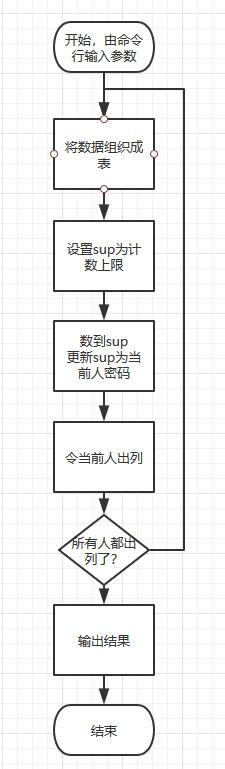
\includegraphics[scale=0.7]{process.jpg}
		\caption{基本算法思路}
		\label{process}
	\end{figure}\par
	本实验中,使用两种数据结构来分别实现任务,即循环链表和线性表。下分类论之。
	\subsection{循环链表}
	\subsubsection{数据类型的定义}
	有循环链表与循环链表的结点。
	\subsubsection{主程序流程}
	主程序读入命令行数据,若发现异常则向用户请求重新输入。此后调用JosephRing循环链表的printAnswer()来输出结果。
	
	\subsection{线性表}
	\subsubsection{数据类型的定义}
	有线性表的节点,及用数组表示的线性表。
	\subsubsection{主程序流程}
	主程序读入命令行数据,若发现异常则向用户请求重新输入。此后调用solve()函数,将线性表作为参数传入来输出结果。
	
	
	\section{关键代码讲解}
	由于没有复杂的函数调用关系,故将函数调用关系图略去。\par
	且此处算法设计思路极其简单,即不断往下数人,直到达到上限就让此人出列,如此循环,直至人均出列。
	\subsection{使用循环链表}
	\subsubsection{数据类型的定义}
	1). 结点数据类型定义
	\begin{lstlisting}[language=C++]
	class JosephNode {
	public:
		int index; // 结点序号
		int code; //结点密码
		JosephNode* next; // 下一个结点
		
		JosephNode(int index, int code) : index(index), code(code), next(nullptr) {};
	};
	\end{lstlisting}
	2). 循环链表数据类型定义
	\begin{lstlisting}[language=C++]
	class JosephRing {
	public:
		int num; // 总结点数
		int sup; //计数上限
		JosephNode* cur; //当前指向结点
		JosephNode* beforeCur; //当前指向结点的前一个结点
		JosephRing(int num, int sup, int* codes);
		void printAnswer();
	};
	\end{lstlisting} 
	\subsubsection{主要算法}
	主要算法即将流程图内容实现一遍,过程较为简单:\par
	\begin{lstlisting}[language=C++]
	void printAnswer() {
		FILE* f = fopen("answer.txt", "w");
		while (num--) {
			sup--;
			//不断数下去,直到数完了上限
			while (sup--) {
				beforeCur = cur;
				cur = cur->next;
			}
			cout << cur->index << ' ';
			fprintf(f, "%d ", cur->index);
			sup = cur->code;
			beforeCur->next = cur->next;
			JosephNode* toDelete = cur;
			cur = cur->next;
			delete toDelete; //删除去掉了的节点占用的内存空间
		}
		cout << endl;
		fprintf(f, "\n");
	}
	\end{lstlisting} 
	
	
	\subsection{使用线性表}
	\subsubsection{数据类型的定义}
	1). 结点数据类型定义
	\begin{lstlisting}[language=C++]
	class JosephNode {
	public:
		int index; // 结点序号
		int code; // 结点密码
		int nextCur; // 下一个结点的位置
		JosephNode(int index, int code, int nextCur) 
		: index(index), code(code), nextCur(nextCur) {};
	};
	\end{lstlisting}
	
	\subsubsection{主要算法}
	主要算法即将流程图内容实现一遍,过程较为简单:\par
	\begin{lstlisting}[language=C++]
	void solve(int num, int m, JosephNode** list) {
		FILE* f = fopen("answer.txt", "w");
		int beforeCur = num - 1;
		int cur = 0;
		while (num--) {
			m--;
			// 循环数人,直到达到m
			while (m--) {
				beforeCur = cur;
				cur = list[cur]->nextCur;
			}
			cout << list[cur]->index << ' ';
			fprintf(f, "%d ", list[cur]->index);
			m = list[cur]->code;
			list[beforeCur]->nextCur = list[cur]->nextCur;
			cur = list[cur]->nextCur;
		}
		cout << endl;
		fprintf(f, "\n");
	}
	\end{lstlisting} 
	
	3). 关于将命令行读入字符串转化为int型数据的代码\par
	此处使用了sscanf函数来实现\par
	\begin{lstlisting}[language=C++]
	//从字符串中读取一个正整数
	bool tryReadNum(int* dest, char* s) {
		int len = strlen(s);
		for (int i = 0; i < len; i++) {
			if (!isdigit(s[i])) {
				cout << "出现非正整数\n";
				return false;
			}
		}
		sscanf(s, "%d", dest);
	}
	\end{lstlisting}
	
	
	\section{调试分析}
	\subsection{问题发现与解决}
	调试过程中发现设计的循环链表并不能做到循环的效果,而成了单向链表。经Debug模式逐步检验,发现最后未将头结点作为尾结点的下一节点,因而改正。
	
	\subsection{算法的时空复杂度分析}
	假设输入的数据为
	\begin{center}
		$*.exe\ n\ m_{0}\ m_{1}\ \dots\ m_{n}$
	\end{center}\par
	以下分析对循环链表和线性表均有效:\par
	由于算法是一步一步寻找到下一个人来执行的,故显然其时间复杂度为$o(\sum_{i=0}^{n}m_{i})$\par
	此外,空间复杂度上,只需要存储这n个人的密码,序号等信息,故空间复杂度是显然的
	
	\section{代码测试}
	\subsection{data1}
	\fbox{
		\parbox{0.8\linewidth}{
			Input:\\
			约瑟夫环.exe 7 20 3 1 7 2 4 8 4\\
			Output:\\
			6 1 4 7 2 3 5
		}
	}\\
	截图如下:
	\begin{figure}[H]
		\centering
		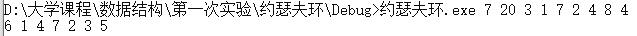
\includegraphics[scale=0.7]{data1.jpg}
		\caption{data1}
		\label{data1}
	\end{figure}\par
	
	\subsection{data2}
	\fbox{
		\parbox{0.8\linewidth}{
			Input:\\
			约瑟夫环.exe 10 50 16 48 35 94 1 6 4 1 9 64\\
			Output:\\
			10 1 9 3 8 2 7 4 6 5
		}
	}\\
	截图如下:
	\begin{figure}[H]
		\centering
		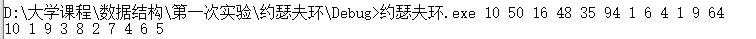
\includegraphics[scale=0.7]{data2.jpg}
		\caption{data2}
		\label{data2}
	\end{figure}\par



	\section{实验总结}
	通过本次的实验,本人更加熟悉了循环链表和线性表的构造和使用,能够更加灵活地运用这两种数据结构来解决问题。此外,还复习了命令行参数的使用,加深了印象。




	\section{附录}
	\subsection{约瑟夫问题(循环链表实现)完整代码}
	\begin{lstlisting}[language=C++]
	#include <iostream>
	#include <cstdio>
	#include <cstring>
	
	using namespace std;
	
	// 约瑟夫循环链表结点
	class JosephNode {
	public:
		int index; //结点序号
		int code; //结点密码
		JosephNode* next; //下一个结点
		
		JosephNode(int index, int code) : index(index), code(code), next(nullptr) {};
	};
	
	// 约瑟夫循环链表
	class JosephRing {
	public:
		int num; // 总结点数
		int sup; // 计数上限
		JosephNode* cur; //当前结点
		JosephNode* beforeCur; //当前结点的前一个结点
		JosephRing(int num, int sup, int* codes) : num(num), sup(sup){
			cur = new JosephNode(1, codes[0]);
			JosephNode* p = cur;
			for (int i = 1; i < num; i++) {
				p->next = new JosephNode(i + 1, codes[i]);
				p = p->next;
			}
			beforeCur = p;
			p->next = cur;
		}
	
		// 输出结果
		void printAnswer() {
			FILE* f = fopen("answer.txt", "w");
			while (num--) {
				sup--;
				//不断数下去,直到数完了上限
				while (sup--) {
					beforeCur = cur;
					cur = cur->next;
				}
				cout << cur->index << ' ';
				fprintf(f, "%d ", cur->index);
				sup = cur->code;
				beforeCur->next = cur->next;
				JosephNode* toDelete = cur;
				cur = cur->next;
				delete toDelete; //删除去掉了的节点占用的内存空间
			}
			cout << endl;
			fprintf(f, "\n");
		}
	};
	
	//从字符串中读取一个正整数
	bool tryReadNum(int* dest, char* s) {
		int len = strlen(s);
		for (int i = 0; i < len; i++) {
			if (!isdigit(s[i])) {
				cout << "出现非正整数\n";
				return false;
			}
		}
		sscanf(s, "%d", dest);
	}
	
	int main(int argc, char* argv[])
	{
		bool flag = true;
		// 对命令行参数的数量做分类,要满足题目要求,至少有4个参数
		if (argc >= 4) {
			int* codes = new int[argc - 1];
			// 将命令行参数转化为int类型数据存储在code中
			for (int i = 1; i < argc; i++) {
				if (!tryReadNum(codes + i - 1, argv[i])) {
					flag = false;
					break;
				}
			}
			// 判断人数和密码数是否对应
			if (codes[0] != argc - 3 && flag) {
				cout << "人数或密码数有误\n";
				flag = false;
			}
			if (flag) {
				// 实例化JosephRing,调用其printAnswer()方法以完成题目
				JosephRing* jr = new JosephRing(codes[0], codes[1], codes + 2);
				jr->printAnswer();
			}
		}
		if(!flag) {
			// 命令行参数格式不正确,要求重新输入。
			int num, m;
			cout << "命令行信息不完整,请重新输入,按照如下格式:\n"
			<< "〈人数n〉〈初始的报数上限m〉〈密码1〉 …… 〈密码n〉\n" << endl;
			cin >> num >> m;
			int* codes = new int[num]; 
			for (int i = 0; i < num; i++) {
				cin >> codes[i];
			}
			// 实例化JosephRing,调用其printAnswer()方法以完成题目
			JosephRing* jr = new JosephRing(num, m, codes);
			jr->printAnswer();
		}
	}
	\end{lstlisting}
	
	
	
	\subsection{约瑟夫问题(线性宝实现)完整代码}
	\begin{lstlisting}[language=C++]
		#include <iostream>
		#include <cstdio>
		#include <cstring>
		
		using namespace std;
		
		// 约瑟夫结点
		class JosephNode {
		public:
			int index; //结点序号
			int code; //结点密码
			int nextCur; //下一个结点的位置
			JosephNode(int index, int code, int nextCur) 
			: index(index), code(code), nextCur(nextCur) {};
		};
		
		// 从字符串s中读取正整数,存入dest中
		bool tryReadNum(int* dest, char* s) {
			int len = strlen(s);
			for (int i = 0; i < len; i++) {
				if (!isdigit(s[i])) {
					cout << "出现非正整数\n";
					return false;
				}
			}
		sscanf(s, "%d", dest);
		return true;
		}
		
		// 解约瑟夫问题
		void solve(int num, int m, JosephNode** list) {
			FILE* f = fopen("answer.txt", "w");
			int beforeCur = num - 1;
			int cur = 0;
			while (num--) {
				m--;
				// 循环数人,直到达到m
				while (m--) {
					beforeCur = cur;
					cur = list[cur]->nextCur;
				}
				cout << list[cur]->index << ' ';
				fprintf(f, "%d ", list[cur]->index);
				m = list[cur]->code;
				list[beforeCur]->nextCur = list[cur]->nextCur;
				cur = list[cur]->nextCur;
			}
			cout << endl;
			fprintf(f, "\n");
		}
		
		int main(int argc, char* argv[])
		{
			int num, m, code;
			JosephNode** list = nullptr;
			bool flag = true;
			// 对命令行参数的数量做分类,要满足题目要求,至少有4个参数
			if (argc >= 4) {
				// 读取人数
				if (!tryReadNum(&num, argv[1])) {
					flag = false;
				}
				// 判断人数和密码数是否一致
				if (num != argc - 3 && flag) {
					cout << "人数或密码数有误\n";
					flag = false;
				}
				// 读取初始密码
				if (!tryReadNum(&m, argv[2]) && flag) {
					flag = false;
				}
				if (flag) {
					list = new JosephNode*[num];
					// 读取所有密码
					for (int i = 0; i < num; i++) {
						if (!tryReadNum(&code, argv[i + 3])) {
							flag = false;
							break;
						}
						list[i] = new JosephNode(i + 1, code, i == num - 1 ? 0 : i + 1);
					}
					// 执行
					solve(num, m, list);
					return 0;
				}
			}
			if (flag) {
				// 命令行输入信息不完整
				cout << "命令行信息不完整,请重新输入,按照如下格式:\n"
				<< "〈人数n〉〈初始的报数上限m〉〈密码1〉 …… 〈密码n〉\n"
			    << endl;
				// 重新读取人数和初始密码
				cin >> num >> m;
				list = new JosephNode*[num];
				// 重新读取密码
				for (int i = 0; i < num; i++) {
					cin >> code;
					list[i] = new JosephNode(i + 1, code, i == num - 1 ? 0 : i + 1);
				}
				// 执行
				solve(num, m, list);
			}
		}
		
	\end{lstlisting}

\end{document}
